%! Author = Админ
%! Date = 12.03.2022

% Preamble
\documentclass[11pt]{article}
% Packages
\usepackage{amsmath}
\usepackage{graphicx}
\usepackage{gensymb}
\usepackage{mathtools}
\graphicspath{{pictures/}}
% Document
\begin{document}
    \section{Problem}
    \begin{gather*}
        A(2,4,0); B(3,1,1); C(1,1,3); D(0,5,1)\\
        \overline{AB}(1,-3,1); \overline{CD}(-1,4,-2)\\
    \end{gather*}
    a) \newline % crossproduct of AB and CD gives you a normal vector ...
    \[\overline{N}=\overline{AB}\times\overline{CD}=det(\begin{bmatrix}
                                                        \overline{i} & \overline{j} & \overline{k}\\
                                                         1 & -3 &  1 \\
                                                        -1 &  4 & -2
    \end{bmatrix}) = \begin{bmatrix}
                      2  \\
                      1 \\
                      1
    \end{bmatrix} \]
    \[2x-y+z=d\]
    \[d_1=8\]
    . . .


    b) \newline
    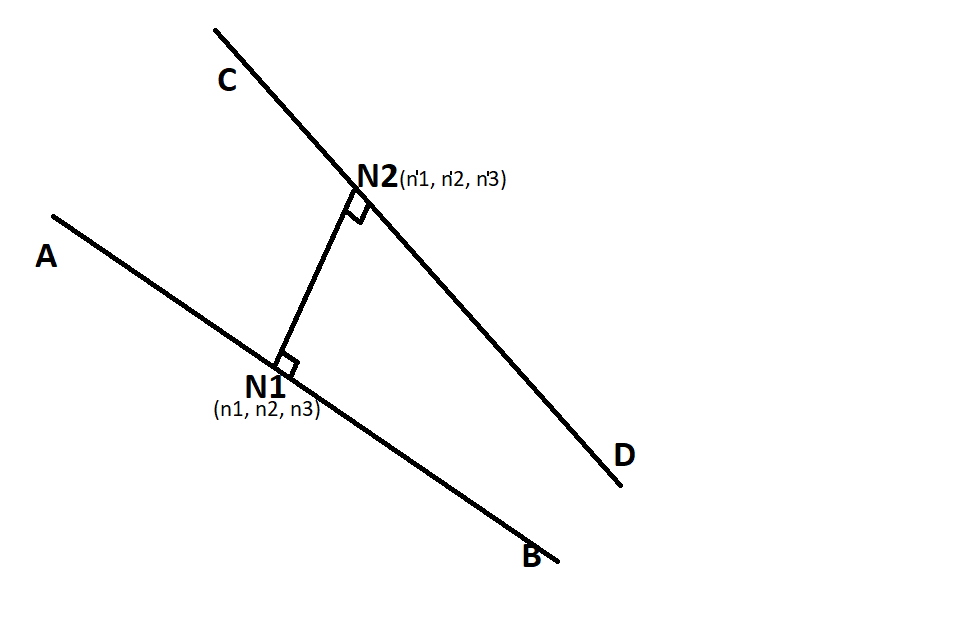
\includegraphics[width=200px]{taskOne.PNG} \newline
    1)
    \[\overline{AB}\cdot\overline{N}=0\]
    \[\begin{cases}
        x(t_1)=t_1+2   \\
        y(t_1)=-3t_1+4 \\
        z(t_1)=t_1     \\
    \end{cases}\]
    \begin{gather*}
        n_1=t_1+2   \\
        n_2=-3t_1+4 \\
        n_3=t_1     \\
    \end{gather*}
    2)
    \[\overline{CD}\cdot\overline{N}=0\]
    \[\begin{cases}
          x(t_2)=-t_2+1  \\
          y(t_2)=4t_2+1  \\
          z(t_2)=-2t_2+3 \\
    \end{cases}\]
    \begin{gather*}
        n_1^\prime=-t_2+1  \\
        n_2^\prime=4t_2+1  \\
        n_3^\prime=-2t_2+3 \\
        \overline{N_1N_2}(-t_2-t_1-1; 4t_2-3+3t_1; -2t_2-t_1+3)\\
    \end{gather*}
    \[\begin{cases}
          \overline{AB}\cdot\overline{N_1N_2}=0  \\
          \overline{CD}\cdot\overline{N_1N_2}=0  \\
    \end{cases}\]
    \[\begin{cases}
          -15t_2-11t_1+11=0  \\
          21t_2+15t_1-17=0  \\
    \end{cases}\]
    \begin{gather*}
        t_1=-4\\
        t_2=3\frac{2}{3}\\
        \overline{N_1N_2}(-\frac{2}{3}, -\frac{1}{3}, -\frac{1}{3})\\
        \overline{|N_1N_2|}=\sqrt {\frac{2}{3}}\\
    \end{gather*}


    \section{Problem}
    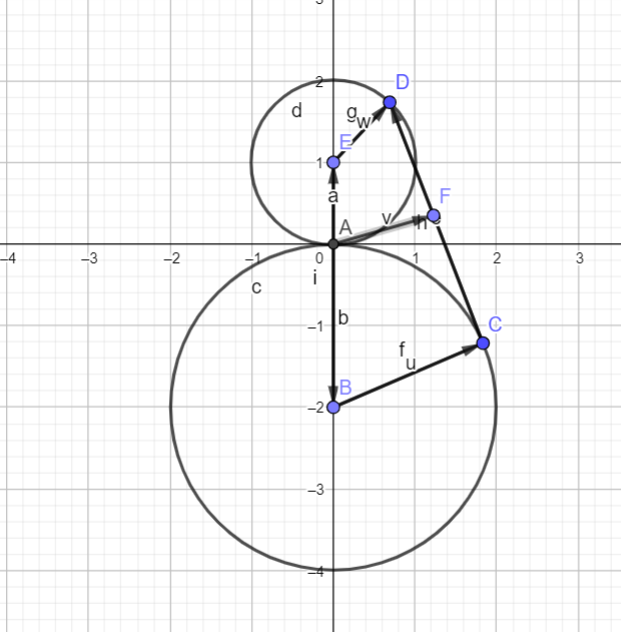
\includegraphics[width=200px]{coord3.PNG} \newline
    a) \newline
    \begin{gather*}
        \overline{AF}(t)-?\\
        \overline{AF}=\overline{AB}+\overline{BC}+\frac{\overline{CD}}{2}\\
        \overline{CD}=\overline{AE}+\overline{ED}-\overline{AB}-\overline{BC}\\
        \overline{AF}=\frac{\overline{AB}+\overline{BC}+\overline{AE}+\overline{ED}}{2}\\
        t_2=2t_1 \\
        \overline{AB}(0,2); \overline{BC}(2\sin{t}, -2+2\cos{t}); \overline{AE}(0, 1); \overline{ED}(\sin{2t}, 1-\cos{2t})\\
        \overline{AF}(2\sin{t}, \cos{t}+1-\frac{\cos{2t}}{2})\\
        x(t)=2\sin{t}\\
        y(t)=\cos{t}+1-\frac{\cos{2t}}{2})\\
    \end{gather*}



\end{document}